多开关匹配是我发明的一个简单的强化学习环境,其主要的环境描写如下:

\begin{definition*}{环境描述}
\# 问题描述

    设计一个多开关匹配的强化学习环境。在该环境中,智能体的任务是通过一系列操作将开关的状态调整到目标状态。每个开关有两个可能的状态:开 (\(1\)) 或关 (\(0\))。智能体可以独立地控制每个开关的状态,置 \(1\) 代表拨动开关,置 \(0\) 代表不对开关进行操作。智能体的目标是通过最少的步骤将所有开关的状态与目标状态一致。
\end{definition*}

\subsection{使用 \textsf{spaces.MultiBinary} 构建组合构建的观测空间和动作空间}

对于这个环境,假设我们需要同时操作 \(3\) 个动作,我们需要注意的是如何构建多个动作空间构成的环境。
在这里,我们直接使用 \textsf{spaces.MultiBinary},并且官方给了一个例子。
\begin{minted}[fontsize=\small, breaklines]{python}
>>> from gymnasium.spaces import MultiBinary
>>> observation_space = MultiBinary(5, seed=42)
>>> observation_space.sample()
>>> array([1, 0, 1, 0, 1], dtype=int8)
>>> observation_space = MultiBinary([3, 2], seed=42)
>>> observation_space.sample()
>>> array([[1, 0],
           [1, 0],
           [1, 1]], dtype=int8)
\end{minted}
我们只要通过其中一个参数的大小,就可以控制这个二进制空间了。
假定我们的开关一共有 \texttt{num\_switches} 个,所以:
\begin{minted}[fontsize=\small, breaklines]{python}
self.observation_space = spaces.MultiBinary(num_switches)
self.action_space = spaces.MultiBinary(num_switches)
\end{minted}
并且通过随机设置一个目标状态,来构建我们的目标:
\begin{minted}[fontsize=\small, breaklines]{python}
self.target_state = np.random.randint(0, 2, size=num_switches)
\end{minted}
对于动作,通过 \(1\) 表示拨动开关,\(0\) 表示不拨动开关,这个在 \textsf{step} 函数中的核心逻辑为:
\begin{minted}[fontsize=\small, breaklines]{python}
self.target_state = np.random.randint(0, 2, size=num_switches)
self.state = (self.state + action) % 2
\end{minted}

\subsection{可视化展示}

我们的环境也做了一个简单的可视化(如图~\ref{fig:multiswitch-env-render}),具体代码实现需要参考代码中的 \textsf{render} 函数。

\begin{figure}[htbp]
    \centering
    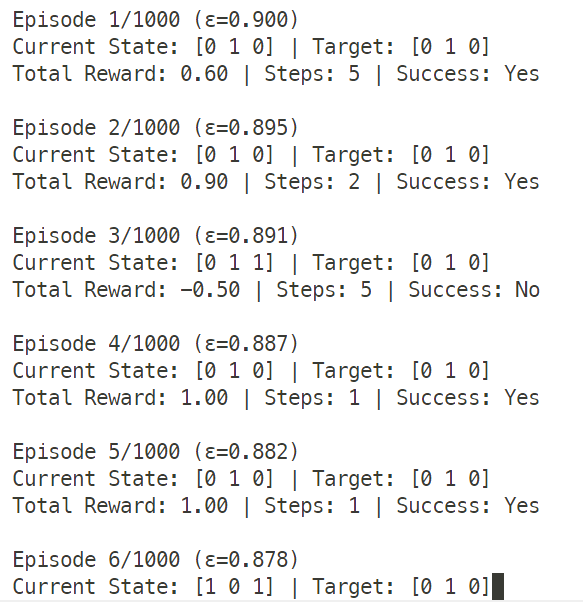
\includegraphics[width=0.5\textwidth]{figure/multi-switch-env_render1.jpg}
    \caption{扫地机器人学习过程可视化展示(\textsf{render} 函数实现)}\label{fig:multiswitch-env-render}
\end{figure}

\subsection{实现代码}

对于多开关匹配的环境的具体代码,请参考附录~\ref{sec:multi-switch-env}。